\section{Introduction}
The filevisitor.py script, found in Listing \ref{listing:filevisitor}, was used to complete the bulk of the work in completing these exercises.  The scripts main function is to search the collection for documents and then perform some operations on each depending on its configuration.  It is used to determine word and bigram counts (Question 4.1), vocabulary size and growth (Question 4.2), in-link count (Question 4.8) and build an inverted index for the document collection (Question 5.8).

In addition to the filevisitor.py script two R scripts (buildgraphs.R, found in Listing \ref{listing:buildgraphs}, and graphvocab.R, found in Listing \ref{listing:graphvocab}), were used to create the graphics used for each exercise.

Finally, to demonstrate the completed inverted index for exercise 5.8, the search.py script was created.  This script can be found in Listing \ref{listing:search}.

\section{Question 4.1}

\subsection{Question}
Plot rank-frequency curves (using a log-log graph) for words and bigrams in the Wikipedia collection available through the book website ( http://www.search-engines-book.com ). Plot a curve for the combination of the two. What are the best values for the parameter c for each curve?

\subsection{Approach}
The \texttt{FileVisitor} class found in Listing \ref{listing:filevisitorclass} recursively searches the directories of the Wikipedia collection.

\lstinputlisting[language=Python, caption={The FileVisitor Class}, label=listing:filevisitorclass,linerange={15-44},firstnumber=15]{code/filevisitor/filevisitor.py}

As it finds files it performs various operations on those files to complete the different tasks required to complete the selected exercises.  This is done by calling the \texttt{counter.count} method, found on line 33.

\clearpage

The BeautifulSoup library \cite{py:beautifulsoup} was used to remove the HTML tags, and then the NLTK library \cite{py:nltk} was used to tokenize the text.  Each word was then counted manually using the \texttt{count} method of the WordCounter class, found in Listing \ref{listing:wordcounter}, and the \texttt{bigram} method of the NLTK library \cite{py:nltk} was used to count the bigrams.  The \texttt{results} method then wrote these counts to a file which was used to create the resulting graphs.

\lstinputlisting[language=Python, caption={The WordCounter Class}, label=listing:wordcounter,linerange={46-97},firstnumber=46]{code/filevisitor/filevisitor.py}

\clearpage

\subsection{Results}
The \texttt{buildgraph.R} script, found in Listing \ref{listing:buildgraphs}, was used to create the following graphs.  The word count graph can be found in Figure \ref{fig:wc}, the bigram count graph can be found in Figure \ref{fig:bigram}, and the graph showing the combination of the two can be found in Figure \ref{fig:both}.

\begin{figure}[h!]
\centering
\label{fig:wc}
\fbox{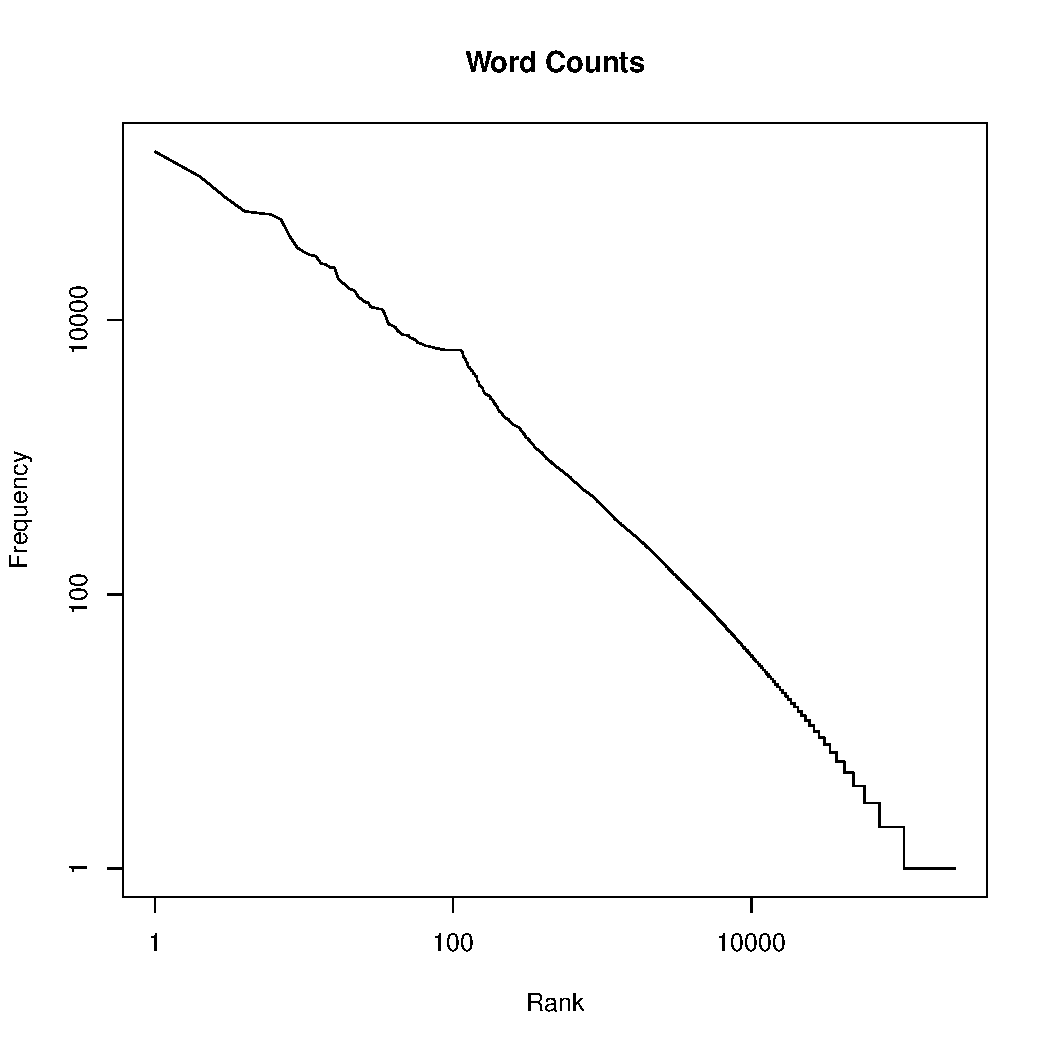
\includegraphics[scale=.55]{code/Rscripts/wc.pdf}}
\caption{Word Counts for Small Wikipedia Corpus}
\end{figure}

\begin{figure}[h!]
\centering
\label{fig:bigram}
\fbox{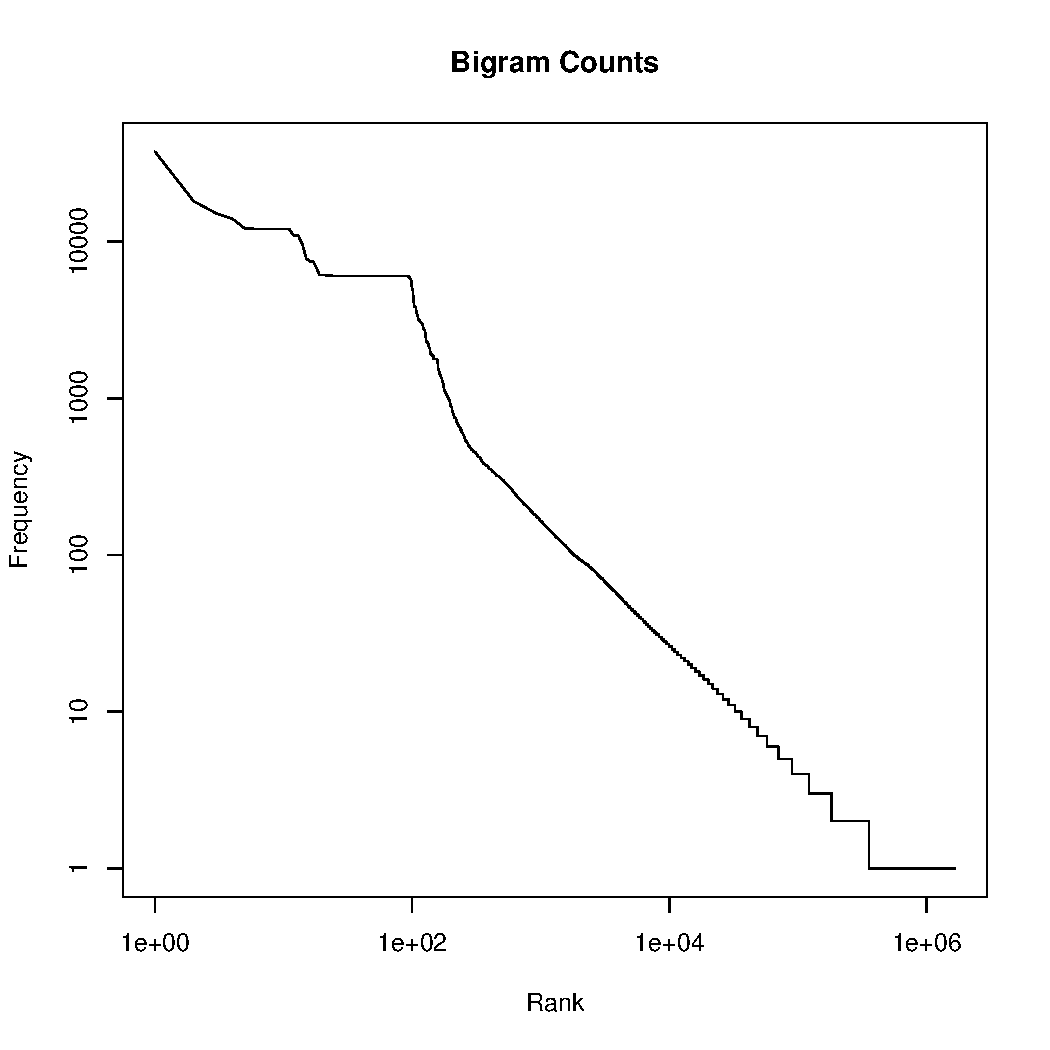
\includegraphics[scale=.55]{code/Rscripts/bg.pdf}}
\caption{Bigram Counts for Small Wikipedia Corpus}
\end{figure}

\begin{figure}[h!]
\centering
\label{fig:both}
\fbox{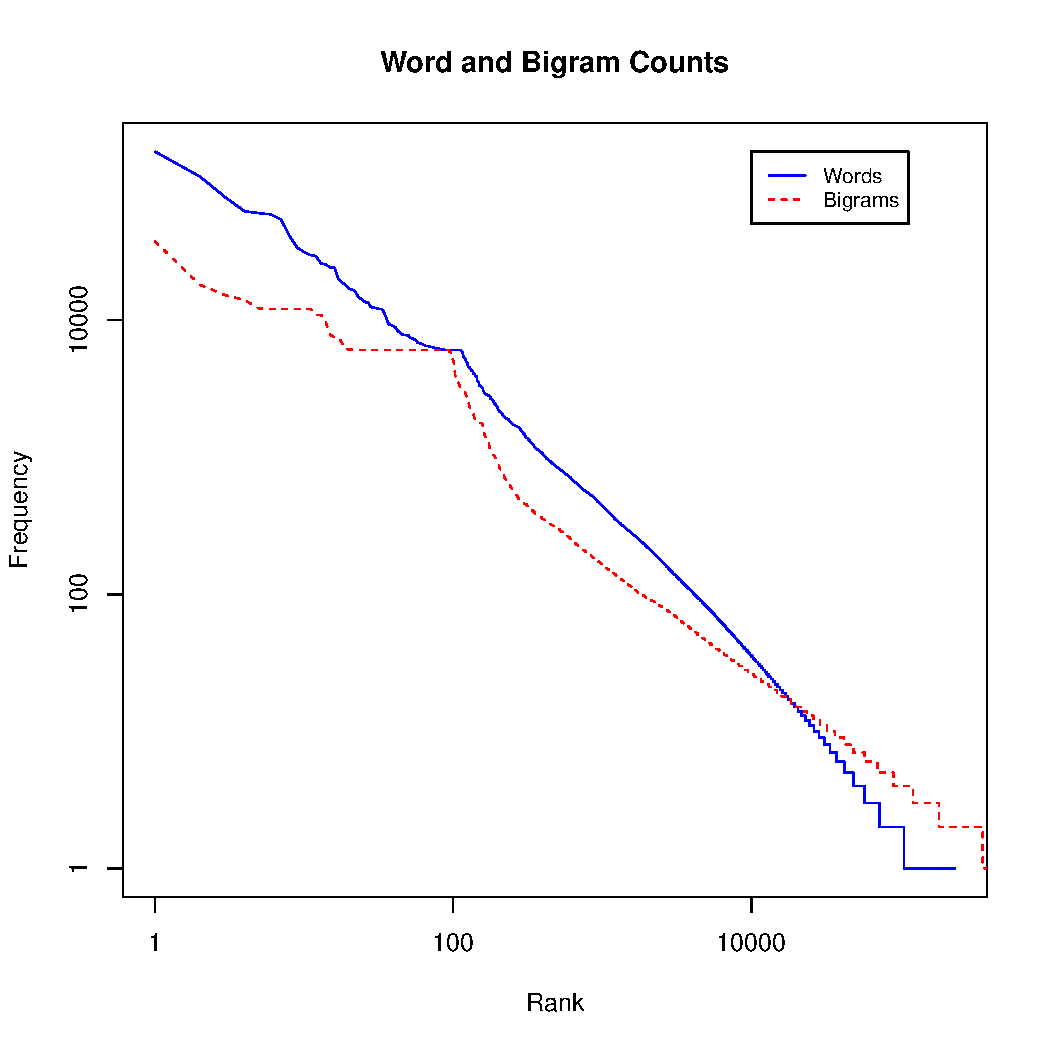
\includegraphics[scale=.55]{code/Rscripts/both.pdf}}
\caption{Both Word and Bigram Counts for Small Wikipedia Corpus}
\end{figure}
